\documentclass{article}

\usepackage[margin=1in]{geometry} 
\usepackage{amsmath,amsthm,amssymb,hyperref, multicol, tikz, romannum, wrapfig}
\usetikzlibrary{arrows.meta, positioning}
\usepackage[framemethod=tikz]{mdframed}



\newcounter{result}[section]
\setcounter{result}{0}



\newenvironment{result}[4]{
  \refstepcounter{result}

  \mdfsetup{
    frametitle={
      \tikz[baseline=(current bounding box.east),outer sep=0pt]
        \node[anchor=east,rectangle,fill=#4!20]
        {\strut #1~#2.\arabic{result}:~#3};
    },
    innertopmargin=10pt,
    linecolor=#4!20,
    linewidth=2pt,
    topline=true,
    frametitleaboveskip=\dimexpr-\ht\strutbox\relax
  }

  \begin{mdframed}\relax \begin{center}
}{
  \end{center} \hfill \end{mdframed} \vspace{3\baselineskip}
}

\hypersetup{colorlinks=True, linkcolor=cyan}



\newcommand{\R}{\mathbb{R}}  
\newcommand{\Z}{\mathbb{Z}}
\newcommand{\N}{\mathbb{N}}
\newcommand{\Q}{\mathbb{Q}}

\newcommand{\suc}{\!+\!\!+\!}

\newcommand{\ZF}{\mathcal{ZF}}



\begin{document}
\pagenumbering{arabic}


\title{Tao Analysis - My Visualisations and Proofs}
\author{Rhitt C}

\maketitle
\tableofcontents

\pagebreak

\setlength{\parskip}{8pt}
\section{Abstract, Motivation and Preliminaries}

\subsection{Abstract}

I decided to write this text as a means to consolidate my personal understanding of undergraduate Real Analysis, 
and also to practise the skill of writing academic papers. 

It is heavily inspired and guided by Terrence Tao's Analysis Vol. \Romannum{1} and \Romannum{2}.
However, I have taken many liberties in altering formulations to my liking, 
completely spelling out motivating arguments before most definitions and theorems (even if this makes it clunky at times), 
going on large digressions, and providing visuals.
I'm also including my solutions to the exercises in Tao's texts, mainly for personal reference.

As a digression on expression, in aspiration of approbation from Big M's appellation upon examination, the language register is largely formal in an attempt to adhere to writing conventions. But we undergo register shifts towards 
informality where appropriate, particularly in avoiding the infamous passive voice\footnote{why is this even a scientific convention smh ts pmo}. This is because it would unnecessarily restrict syntactic freedom 
in a situational context where it is the \textit{content} that matters far more than the expression. Thus, it is more favourable to be able to convey the content precisely and elegantly without jumping though linguistic hoops every step of the way.

\subsection{Why do Analysis? - Motivation 1}
The motivation for Analysis is twofold:

Firstly, the most obvious reason is to understand deeper concepts that stray far from the base intuition you get from VCE and high school in general.
For example, you may have heard the result that there are more $x\in\R$ with $x\in(0, 1)$ than there are $p\in\Q$ with $p\in(-\infty, \infty)$\footnote{the precise statement is with a concept called \textit{cardinality}}.
Your intuition tells you this is absurd, because clearly both are infinite! How can we have $\infty_1>\infty_2$?
Even more counterintuitive is that there are \textit{just as many} $n\in\N$ as there are $x\in\Z$, even though clearly for every $n\in\N$ there are both $\pm n\in\Z$,
and so you'd expect there to be about twice as many integers as there are naturals.
It seems like mathematicians are just making stuff up at this point.
But in Real Analysis, we handle $\infty$ \textit{rigorously} to make such statements not only meaningful, but to fully understand the motivation for even discussing such matters in the first place.
The full level of rigour makes many theorems feel discoverable, in that you properly understand how you would derive and prove them in the first place.

We will see how it answers exactly what you can and can't do with $\infty$. E.g. Consider the matrix 
$$ M = \begin{pmatrix}
    1   & 0     & 0           & \cdots \\
    -1  & 1     & 0           & \cdots \\
    0   & -1    & 1           & \cdots \\
    0   & 0     & -1          & \cdots \\
    \cdots & \cdots  & \cdots & \ddots
\end{pmatrix} $$
You'd expect the sum of all elements $\sum M_{ij}$ to be the same either way, whether you sum over rows or over columns first.
But we have, if you'll excuse the lax notation, $$\sum_{\text{over rows first}} M = \sum_{\text{over columns}} \begin{pmatrix}1\\0\\0\\\vdots\end{pmatrix}=1,\qquad \sum_{\text{over columns first}} M = \sum_{\text{over rows}} \begin{pmatrix}0 & 0 & 0 & \cdots \end{pmatrix}=0$$
$$\therefore \left(\sum_{\text{over rows first}} M =1\right)\quad\neq\quad\left(\sum_{\text{over columns first}} M =0\right)$$

So we have illustrated that you can't always interchange the order in which you sum infinitely many numbers, contrary to intuition.
Real Analysis gives the full derivation for the precise conditions in which you can safely do so\footnote{see Fubini}.
As we have seen, it teaches you how to properly deal with $\infty$.
So in a sense, Real Analysis can make you like \textit{The Man Who Knew Infinity}\footnote{cold, cold, cold}.

More than that, Real Analysis answers to the highest echelon that is possible with logic (provably so, in fact) the \textit{why} behind essentially everything you've ever been taught in maths from kindergarten to high school, leave some small details about $\mathbb{C}$.
You realise the true degree of freedom that maths gives you.
And you learn complete objectivity.
You don't have to take anyone's word for it, just prove it yourself.
You learn to make a statement, and the proof of it, so damn precise that there is \textit{zero} ambiguity or subjectivity in it; I say this without hyperbole.
Doesn't matter if a teacher thinks your expression is lacking; you can be \textit{absolutely sure} that your statement is correct, given you're subtle enough with what is meant by correct.

\subsection{Why do Analysis? - Motivation 2 (very important)}

Secondly, we will see how blindly following the whims of what our intuition deems reasonable can very easily lead to contradiction. 
The many times that this occurred historically, there was great philosophical anguish about what assumptions to keep and what to discard, substantially impeding on mathematical progress. 

\begin{wrapfigure}{r}{0.1\textwidth} \centering 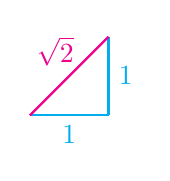
\begin{tikzpicture}
    \draw[cyan, thick] (0, 0) -- node[midway, below] {$1$} (1, 0);
    \draw[cyan, thick] (1, 0) -- node[midway, right] {$1$} (1, 1);
    \draw[magenta, thick] (1, 1) -- node[midway, left=5pt, above] {$\sqrt{2}$} (0, 0);
\end{tikzpicture} \end{wrapfigure}
For example, take $\sqrt{2}$, a quantity that arises in geometry very naturally as the length of the hypotenuse in a triangle with both other side lengths $1$.
In ancient Greece, many held the worldview that everything in the real world, like this hypotenuse, can be quantified as a rational number in $\Q$.
And they held this assumption to be so blatantly obvious that it underpinned their philosophy of everything from music to the universe itself.
So when it was found that $\sqrt{2}\in\Q$ would imply a contradiction, even though the triangle is very much real, it led to a crisis in which many ancient Greeks had to reevaluate their entire philosophy.

Because we've been taught from a young age that irrational numbers exist and do indeed show up in the real world, we now find the concept to be no doubt very intuitive. 
But how can we be absolute \textit{sure} that there isn't some other cancerous contradiction hiding somewhere in our mathematical foundations as well, just waiting to spread into everything we think we know, as it did for the Greeks?
The truth is, we're \textit{not} sure. And it's in fact been \textit{proven}\footnote{see G\"odel's Incompleteness Theorems} that we we can never be sure. 
Not unless we rob ourselves of the ability to do primary school arithmetic, which would be very absurd. So as we shall see, we do the next best thing: minimise our set of assumptions to the bare minimum that is still feasible.

To be clear, the issue isn't with logic itself. As a rather lengthy aside, the question of whether logic is valid is philosophical in nature, and seemingly can't ever have a definitive resolution.
For example, it could very well be the case that we and our fictitious universe only exist in the incoherent dream of a butterfly. If so, logic as we perceive it only \textit{appears} valid to us,
yet completely wrong to a scientist observing the dream from outside in the real world. But even though such fundamental questions about reality may be interesting, 
doubting logic every step of the way puts overly restrictive bounds on what mathematical progress is possible.
So they're for the philosopher to ponder over. Instead, the mathematician prescribes a handful of intuitive operations on True/False valued statements, which formalise pure logic. E.g.
\begin{align*} &\text{(True }\&\text{ True) is True, but} \\ &\text{(True }\&\text{ False) is False, as True and False are said to contradict each other.} \end{align*}
Then they prescribe a few more rules on how to produce those logical statements from free variables (which can be mathematical objects), completing the formal, objective link from logic to maths.
E.g.
\begin{align*} ((\forall x, P(x))\implies P(0)\text{) is True} \end{align*}
Finally, they combine all of this into a rulebook which they call the formal logic. Confident that the logic reflects reality, they hand it over to the philosopher to question the validity of.
The mathematician is now happy to accept their logic as absolute and instead ponders questions about how the logic actually affects mathematical statements (theorems, lemmas, corollaries, etc.). 
And even if the philosopher someday finds that the logic is only valid in the dream of a butterfly and invalid outside of it, much of the work done by mathematicians could very well still be moulded to adhere to whatever rulebook is followed by the world outside the dream.

Now that we have set our logic in stone, how do we proceed?
Logic can only tell us about the relationships between logical statements, but makes no comment about many individual statements involving free variables.
E.g. we can show $$\text{(I am a lazy person \& all lazy people are monkeys)}\implies\text{(I am a monkey)}\footnote{given this is stated in a way that avoids mentioning sets}$$
as a whole is True directly from our logic, but we can't individually show that (I am a lazy person) or (all lazy people are monkeys) are True with logic alone because of the free variables (I), (lazy person/people) and (monkey(s)).
And if either of those two statements turn out to be False, then we have no information about whether (I am a monkey) is True or False. I could very well be a monkey despite not being lazy. Thus, all in all, we have an ($\implies$) statement that is True but we can't show definitively that its implication (I am a monkey) is also True\dots which is a good thing because I'm pretty confident I'm not a monkey (but can I \textit{show} definitively that I'm not? Once again, no). 

This is a necessary tradeoff we made so the mathematician will never have to doubt this barebone logic.

So how do we prove a conjecture $P$? 
Instead of the fool's errand of looking for whether $P$ is definitively True,
we loosen our standards slightly and instead show the truth of an ($\implies$) statement as follows: if we accept a base few assumptions, which we call our \textit{axioms}, then $P$ is True.
That is, our standard of proof for $P$ is of the form:
$$Axiom_1\;\&\;Axiom_2\;\& Axiom_3\;\&\;\dots\quad\implies\quad P$$



As a concluding remark, we do not deny the value of intuition. In fact, intuition is absolutely essential for \textit{developing} a conjecture and motivating why it might be plausible. 
Without it we are stuck running a fool's errand of perpetual guess and check, never able to come up with something original and insightful.
But once we are confident that our conjecture is indeed plausible, we \textit{need} to follow a gold standard of proof independent of intuition.
It's the best way we know of to minimise the chance as much as feasible
for a contradiction to sneak up on us from a single far-reaching result we prematurely took as granted long ago. 
That would shatter the foundations of mathematics, much like the contradictory assumption $\sqrt{2}\in\Q$ did for the Greeks. 
Of course, in perhaps the greatest failure of modern maths, we've shown logically that we still can't ever completely eliminate that possibility, 
so long as we demand our axioms be strong enough for maths to be of value.
Nonetheless, mathematicians collectively agree on a handful of axioms called $\ZF$\footnote{there is another axiom called Choice we will explore in Chapter 8 that together with $\ZF$ forms $\ZF \mathcal{C}$, a slightly weaker standard of proof, but we will see that it is in many respects equivalent to $\ZF$ for our purposes} on ``sets'' (all of which we will encounter in the next 2 chapters) as the basis for our gold standard of proof, 
as it's the best that we can feasibly do, and it seems unlikely that it'll ever truly see a contradiction.

The gold standard we set is hence:
\begin{result}{Definition}{G}{The Gold Standard of Proof}{green}
    A conjecture $P$ is considered ``proven'' \textit{if and only if} we can show with our logic that:

    $\ZF \implies P$

\end{result}



\subsection{Logic Preliminaries}
\newcommand{\tr}{\mathcolor{cyan}{\mathfrak{T}}}
\newcommand{\fa}{\mathcolor{magenta}{\mathfrak{F}}}
\newcommand{\ill}{\mathcolor{brown}{\mathfrak{I}}}

This subchapter is mainly for reference in case we wish to clarify logical definitions and their motivations.\footnote{our formulation is only first order, but this is sufficient for our purposes}

Define a statement as a logical object that takes on either $\tr$ (True), $\fa$ (False) or $ \ill $(Ill-Formed),
where $\ill$ indicates the statement is left undefined and considered to have no truth value (e.g. $\frac{1}{0}=1$). 
This way, we have a mechanism to handle ill-formed statements in case they slip through our fingers somewhere down the line.

Also note that by default we define ($S_1 \implies S_2$) to be $\tr$ whenever $S_1$ has a truth value other than $\tr$.
The motivation is simply that it makes things easier to show. 
Under this definition, if we want to show that ($S_1\implies S_2$) as a whole is $\tr$,
 all we need to do is consider the case where $S_1$ is $\tr$ and follow logical arguments that lead to $S_2$'s truth. 
 There is no need to consider when $S_1$ is $\fa$ or $\ill$, making arguments significantly less cluttered.
If you do not agree with this decision, you can of course define it otherwise, but you will soon realise how unnecessarily messy every single proof becomes.

Furthermore, an ($\implies$) statement only comments about \textit{correlation}, not \textit{causation}.
 So you could satisfy (pigs can fly $\implies$ the stock market will crash in $2142$) if pigs can't fly or if somehow both are true, even if there's no causal link between the two individual statements (I doubt flying pigs alone would cause the stock market to crash).
 This is because causality can be an exceedingly philosophically subjective concept (do I think because I am or am I because I think?), and so logic doesn't concern itself with it.
 Note that we don't mean causality in the relativistic sense, which would be a completely different concept.

\begin{result}{Definition}{L}{Operations on Statements}{green}
    Given a statement $S$, the new statement ($not S$) can be formed as follows:
    
    \begin{tabular}{c | c}
        $S$ & $notS$ \\ \hline
        $\tr$ & $\fa$ \\ 
        $\fa$ & $\tr$ \\ 
        $\ill$ & $\ill$
    \end{tabular}
    
    
    Given two statements $S_1$ and $S_2$, new statements ($S_1\&S_2$) and ($S_1\implies S_2$) can be formed as follows:

    \begin{tabular}{c c | c | c}
        $S_1$ & $S_2$
        & $S_1 \& S_2$
        & $S_1 \implies S_2$ \\ \hline

        $\tr$ & $\tr$
        & $\tr$ & $\tr$ \\

        $\tr$ & $\fa$
        & $\fa$ & $\fa$ \\ \hline

        $\fa$ & $\tr$
        & $\fa$ & $\tr$ \\

        $\fa$ & $\fa$
        & $\fa$ & $\tr$ \\ \hline

        $\tr$ & $\ill$
        & $\ill$ & $\ill$ \\

        $\ill$ & $\tr$
        & $\ill$ & $\tr$ \\ \hline

        $\fa$ & $\ill$
        & $\ill$ & $\tr$ \\

        $\ill$ & $\fa$
        & $\ill$ & $\tr$ \\ \hline

        $\ill$ & $\ill$
        & $\ill$ & $\tr$
    \end{tabular}


    Given two statements $S_1$ and $S_2$, new statements ($S_1orS_2$), ($S_1\impliedby S_2$), ($S_1 \iff S_2$) can be formed as follows:
    
    $\begin{aligned}
        (S_1 or S_2) & \text{ has the same truth value as } (not(not S_1\;\; \&\;\; not S_2)) \\
        (S_1 \impliedby S_2 ) & \text{ has the same truth value as } (S_1 \implies S_2) \\ 
        (S_1 \iff S_2 ) & \text{ has the same truth value as } ((S_1 \impliedby S_2 ) \;\;\&\;\; (S_1 \implies S_2))
    \end{aligned}$

\end{result}



\pagebreak
\section{Construction of $\N$}

\setcounter{subsection}{-1}
\subsection{The Peano Axioms - Motivation for Defining $\N$ Axiomatically}
We first motivate the set of naturals $\N = \{0, 1, 2, \dots\}$ to be so essential to maths that it deserves its own few axioms.

As mentioned, $\ZF$, the ultimate handful of axioms we are leading up to, lay out what is legally a set. So what even is a set intuitively? Informally, a set $S$ is the collection of all objects $x$ satisfying a certain predicate\footnote{see 1.4 Logic Preliminaries} $P_S[x]$. That is,
$$ x \in S \iff P_S[x]$$
In fact, if we could take that informal definition as our axiom, then would be basically done! That alone would imply 7 out of 8 $\ZF$ Axioms.
But alas, it's too good to be true. We will see in the next chapter that such an axiom would allow for certain infinitely large sets that lead to contradictions.
But the resolution isn't to completely reject the notion of $\infty$ itself, as we still very much need it to derive many rich and powerful results everywhere from number theory to calculus and beyond.
So instead, we handle $\infty$ very subtly.

The most basic form of $\infty$ is that of ``counting numbers'', which we will formalise into the set $\N = \{0, 1, 2, \dots\}$. Informally speaking, is there a counting number out there that you can't count past?
No! You've no doubt had fun with this as a child. You compete with your friend to see who can think up the biggest number imaginable. Whatever $n$ they think up, you respond swiftly with $n+1$.
This is a property we want for our $\N$, that it doesn't have a maximal element; you can always find a larger one. Infinity in the sense of that property doesn't seem to be contradictory, so we define our $\ZF$ axioms to allow for such an $\N$ to exist.
We will see throughout the text that all other infinite sets such as $\Z, \Q, \R$, and subsequently all other notions of $\infty$, can be constructed directly from $\N$, so we are happy.

We will later see that one of the $\ZF$ Axioms makes reference to all 5 Peano Axioms, but the converse is not true. So we say $\ZF$ contains Peano.
The standard in the literature is actually to not even mention the Peano Axioms at all, but instead condense them into a single, concise axiom in $\ZF$ that satisfies our formulation of Peano \textit{automatically}.
We will not do this, as it is far more intuitive to define Peano first.

\subsection{The Peano Axioms}
We now lay out the requirements that our first infinite ``set'' $\N$ must satisfy as the 5 Peano Axioms. 
As sets have not yet been defined, we primitively let $\N[n]$ be the predicate for whether $n$ is natural, 
substituting for where we would otherwise say $n \in \N$. We abbreviate ($\forall n\;s.t.\; \N[n]$) as ($\forall \N[n]$)


    We start with the bare minimum by demanding that some fixed object, namely $0$, be well defined. $0$ will be crucial to defining a few later axioms, as it gives us a sort of starting point.

    \begin{result}{Axiom}{P}{Existence of 0}{red}

        There exists an object $0$ that is natural and can be used in later axioms.
        $$\exists0\quad s.t.\quad \N[0]\quad\&\quad \text{\textcolor{magenta}{P.3} and \textcolor{magenta}{P.5} are met.}$$

        
\begin{tikzpicture}[scale=1.2]
            \fill[cyan] (0,0) circle (3pt);
            \draw[ultra thick, cyan] (0,-0.2) -- (0, 0.2);
            \node[below, cyan, font=\large] at (0,-0.2) {$0$};
        \end{tikzpicture}

    \end{result}

    \pagebreak

    Now to populate $\N$, we introduce a new primitive operation (which similarly is not truly an operation - it is no more than a suggestive notation for objects otherwise unrelated to $0$) that will later by superseded by addition. We call it \textit{succession}, and it satisfies an axiom of closure as follows.
    It is named closure since you can't ``escape'' the naturals (you are en\textit{closed} in naturals) no matter how many times you take the succession.
    Informally, we hope that it behaves like our intuition for incrementing a number by $1$, and thus forces the infinitely many ``counting numbers" to now be well defined and in $\N$.
    Denote the succession of a natural $n$ as $n\suc$, and label $(1:=0\suc),\; (2:=1\suc),\; (3:=2\suc),\;\dots$


    \begin{result}{Axiom}{P}{Closure of $\N$ under $(\suc)$}{red}
        All naturals have natural successions.
        $$(\forall \N[n]) \quad \N[n\suc]$$

        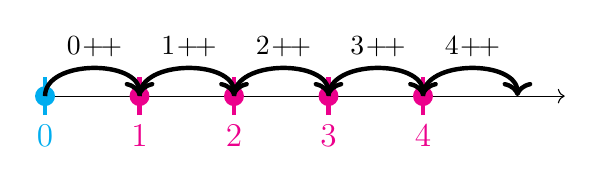
\begin{tikzpicture}[scale=1.2]

            \draw[->] (0,0) -- (5.5, 0);
            \fill[cyan] (0,0) circle (3pt);
            \draw[ultra thick, cyan] (0,-0.2) -- (0, 0.2);
            \node[below, cyan, font=\large] at (0,-0.2) {$0$};

            \fill[magenta] (1,0) circle (3pt);
            \draw[ultra thick, magenta] (1,-0.2) -- (1, 0.2);
            \node[below, magenta, font=\large] at (1,-0.2) {$1$};
            \draw[->, ultra thick] (0,0) to[bend left=90] node[pos=0.5, sloped, above] {$0\suc$} (1,0);

            \fill[magenta] (2,0) circle (3pt);
            \draw[ultra thick, magenta] (2,-0.2) -- (2, 0.2);
            \node[below, magenta, font=\large] at (2,-0.2) {$2$};
            \draw[->, ultra thick] (1,0) to[bend left=90] node[pos=0.5, sloped, above] {$1\suc$} (2,0);

            \fill[magenta] (3,0) circle (3pt);
            \draw[ultra thick, magenta] (3,-0.2) -- (3, 0.2);
            \node[below, magenta, font=\large] at (3,-0.2) {$3$};
            \draw[->, ultra thick] (2,0) to[bend left=90] node[pos=0.5, sloped, above] {$2\suc$} (3,0);

            \fill[magenta] (4,0) circle (3pt);
            \draw[ultra thick, magenta] (4,-0.2) -- (4, 0.2);
            \node[below, magenta, font=\large] at (4,-0.2) {$4$};
            \draw[->, ultra thick] (3,0) to[bend left=90] node[pos=0.5, sloped, above] {$3\suc$} (4,0);

            \draw[->, ultra thick] (4,0) to[bend left=90] node[pos=0.5, sloped, above] {$4\suc$} (5,0);

        \end{tikzpicture}
    \end{result}

    

    However, \textcolor{magenta}{P.1} and \textcolor{magenta}{P.2} alone are not strong enough to force $\N$ to populate with our infinitely many elements.
    In particular, they do not prevent existence of a natural $n$ with $(n\suc)=0$.
    And yet, informally speaking, this means $n$ overflows back to $0$, forming what's called a modulo cycle. As illustrated below (with $n=4$), this only guarantees the existence of $n+1$ naturals. 
    Modulo sets have many applications, but they are not what we desire as a full, infinite set of ``counting numbers'', particularly if that $n$ turns out to be $0$ itself, leading to $0$ trivially being the only guaranteed natural.
    So we explicitly force $\N$ to not be such a modulo cycle by demanding that a natural's succession never overflows back to $0$.

    \begin{result}{Axiom}{P}{$\N$ does not have a modulo cycle overflowing to $0$}{red}
        No natural's succession can be $0$.
        $$(\forall \N[n])\quad (n\suc) \neq 0$$


        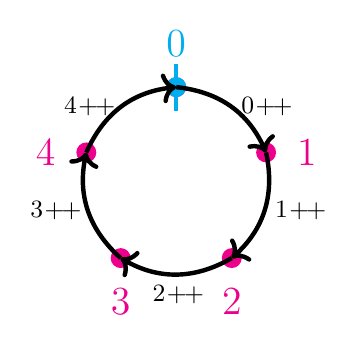
\begin{tikzpicture}[scale=1.2, every node/.style={font=\large, inner sep=1pt}]
            \def\n{5}
            \def\radius{1}

            \foreach \i in {0,...,4} {
                \pgfmathsetmacro{\angle}{90-\i*360/\n}
                \coordinate (N\i) at (\angle:\radius);
                \fill[magenta] (N\i) circle (3pt);
            }
            \fill[cyan] (N0) circle (3pt);

            \draw[ultra thick, cyan] (N0 |- 0,0.75) -- (N0 |- 0,1.25);

            \node[above=10pt, cyan, font=\Large] at (N0) {$0$};
            \node[right=10pt, magenta, font=\Large] at (N1) {$1$};
            \node[below=10pt, magenta, font=\Large] at (N2) {$2$};
            \node[below=10pt, magenta, font=\Large] at (N3) {$3$};
            \node[left=10pt, magenta, font=\Large] at (N4) {$4$};

            \draw[->, ultra thick] (N0) to[bend left=30] node[midway, right, outer sep = 1mm, font=\small] {$0\suc$} (N1);
            \draw[->, ultra thick] (N1) to[bend left=30] node[midway, right, outer sep = 1mm, font=\small] {$1\suc$} (N2);
            \draw[->, ultra thick] (N2) to[bend left=30] node[midway, below, outer sep = 1mm, font=\small] {$2\suc$} (N3);
            \draw[->, ultra thick] (N3) to[bend left=30] node[midway, left, outer sep = 1mm, font=\small] {$3\suc$} (N4);
            \draw[->, ultra thick] (N4) to[bend left=30] node[midway, left, outer sep = 1mm, font=\small] {$4\suc$} (N0);
        \end{tikzpicture}

    \end{result}


    \pagebreak
    As it stands, the issue hasn't been fully resolved yet.
    There is still the pathological case of an \textit{offset} modulo cycle, in which a natural $n$ overflows back so that $(n\suc)=(m\suc)$ even though $(m\suc)$ is already the successor of a different natural $m$.
    An offset modulo cycle once again guarantees only finitely many naturals, which we don't want.
    We now complete our requirements on $(\suc)$ by demanding no such successions are the same. Informally, we make $(\suc)$ \textit{injective} i.e. a one-to-one operation (function).


    \begin{result}{Axiom}{P}{$\N$ has no otherwise offset modulo cycles either}{red}

        Succession is injective (one-to-one). That is, distinct naturals have distinct successions.
        $$(\forall \N[n], \N[m])\quad n \neq m \implies (n\suc) \neq (m\suc)$$

        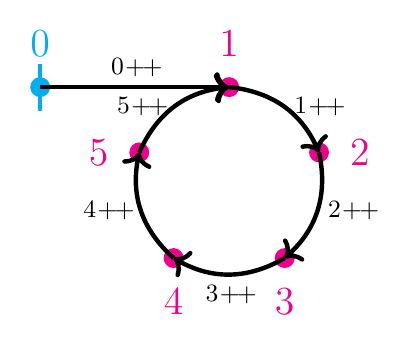
\begin{tikzpicture}[scale=1.2, every node/.style={font=\large, inner sep=1pt}]
            
            \def\n{5}
            \def\radius{1}

            \foreach \i in {0,...,4} {
                \pgfmathsetmacro{\angle}{90-\i*360/\n}
                \coordinate (N\i) at (\angle:\radius);
                \fill[magenta] (N\i) circle (3pt);
            }
            \fill[cyan] (-2, 0 |- N0) circle (3pt);
            \draw[ultra thick, cyan] (-2,0.75) -- (-2,1.25);


            \node[above=10pt, cyan, font=\Large] at (-2, 0 |- N0) {$0$};
            \node[above=10pt, magenta, font=\Large] at (N0) {$1$};
            \node[right=10pt, magenta, font=\Large] at (N1) {$2$};
            \node[below=10pt, magenta, font=\Large] at (N2) {$3$};
            \node[below=10pt, magenta, font=\Large] at (N3) {$4$};
            \node[left=10pt, magenta, font=\Large] at (N4) {$5$};

            \draw[->, ultra thick] (-2, 0 |- N0) to node[midway, above, outer sep = 1mm, font=\small] {$0\suc$} (N0);
            \draw[->, ultra thick] (N0) to[bend left=30] node[midway, right, outer sep = 1mm, font=\small] {$1\suc$} (N1);
            \draw[->, ultra thick] (N1) to[bend left=30] node[midway, right, outer sep = 1mm, font=\small] {$2\suc$} (N2);
            \draw[->, ultra thick] (N2) to[bend left=30] node[midway, below, outer sep = 1mm, font=\small] {$3\suc$} (N3);
            \draw[->, ultra thick] (N3) to[bend left=30] node[midway, left, outer sep = 1mm, font=\small] {$4\suc$} (N4);
            \draw[->, ultra thick] (N4) to[bend left=30] node[midway, left, outer sep = 1mm, font=\small] {$5\suc$} (N0);
        \end{tikzpicture}


    \end{result}


    We now lay out by far the most useful Peano Axiom, which lets us handle the sheer infinite size of $\N$ recursively.
    It is induction, which makes intuitive sense with a domino analogy. 
    Note, induction is not a full logical axiom, as it makes reference to predicates as free variables, which is strictly speaking illegal. 
    This is why it's called an Axiom Schema instead when you want to be logically precise.
    Indeed, it is logically consistent if you consider it to be no more than a template for generating individual axioms for every predicate you need as you go, all of which are themselves well formed logical statements.

    \begin{result}{Axiom Schema}{P}{(PMI) Principle of Mathematical Induction}{red}
    
        If a predicate is met for $0$ (Base Case), and it being satisfied for some natural implies it's met for the succession as well (Inductive Case), then as a domino effect, the predicate is met for all naturals.

        \hfill

        $(\forall P:\rightsquigarrow \{\tr, \fa, \ill\})\qquad(P[0]\;\;\;\&\;\;\;((\forall \N[k])\;P[k]\!\!\implies\!\!P[k\suc])) \quad \implies \quad (\forall \N[n])\; P[n]$

        \vspace{2\baselineskip}

        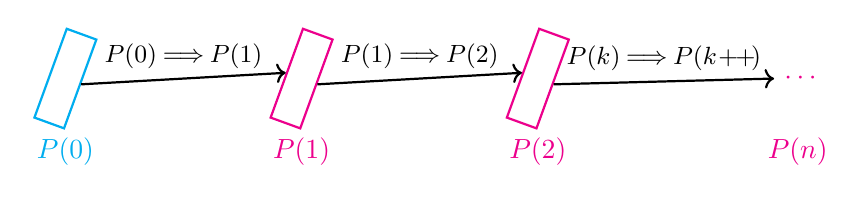
\begin{tikzpicture}[
            dom/.style={rectangle, draw, rotate=-20, minimum width=0.4cm, minimum height=1.2cm, thick},
            arrow/.style={->, thick}
        ]

            \node[dom, cyan] (D1) at (0,0) {};
            \node[below=18pt, cyan] at (D1) {$P(0)$};

            \node[dom, magenta] (D2) at (3,0) {};
            \node[below=18pt, magenta] at (D2) {$P(1)$};

            \node[dom, magenta] (D3) at (6,0) {};
            \node[below=18pt, magenta] at (D3) {$P(2)$};

            \node[below=18pt, magenta] at (9.3, 0) {$P(n)$};


            \draw[arrow] (D1.east) -- node[midway, above, font=\small] {$P(0)\!\!\implies\!\!P(1)$} (D2.west);
            \draw[arrow] (D2.east) -- node[midway, above, font=\small] {$P(1)\!\!\implies\!\!P(2)$} (D3.west);
            \draw[arrow] (D3.east) -- node[midway, above, font=\small] {$P(k)\!\!\implies\!\!P(k\suc)$} (9, 0) node[magenta, right] {$\cdots$};

        \end{tikzpicture}

    \end{result}

    \pagebreak

    We now briefly discuss implications for after $\ZF$ will be well defined. Abstractly speaking, all sets $X$ equipped with an analogous operation $S: X\to X$ (refered to together as an algebraic structure $\langle X, S\rangle$), that obeys the 5 Peano Axioms is said to be \textit{isomorphic} with $\langle\N, (\suc)\rangle$, denoted $\langle X, S\rangle\cong\langle\N, (\suc)\rangle$.
    Note that due to our later discussions only relying on logical implications from the axioms, which are met by $\langle X, S\rangle$, the results we derive must apply to every such isomorphism $\langle X, S\rangle$, given we rewrite our definitions accordingly.
    As such, we do not strictly define a particular $\langle \N, (\suc)\rangle$, but rather refer abstractly to any such solution $\langle X, S\rangle$ to Peano.

    So in a sense, the Peano Axioms lay out a kind of citizenship test, in which $\langle X, S\rangle$ is considered a natural structure if and only if it passes, and it gets all the perks of being a natural citizen that we will now derive.

    \subsection{Addition}
    \subsection{Multiplication}



    \pagebreak
    \section{$\ZF$ Set Theory}
    \setcounter{subsection}{1}
    \subsection{Historical Axioms - Too Good to be True}
    \setcounter{subsection}{0}
    \subsection{$\ZF$ Axioms}
    \setcounter{subsection}{2}
    \subsection{Functions}
    \subsection{Images}
    \subsection{Cartesian Products}
    \subsection{Cardinality}


    \pagebreak
    \section{Constructing $\Z$ and $\Q$}
    \subsection{Constructing $\Z$ - Subtractive Closure of $\N$}
    \subsection{Constructing $\Q$ - Divisive Closure of $\Z$}
    \subsection{Exponentiation of $\Q$ to $\Z$ Powers and the Modulus}
    \subsection{Why $\Q$ is Inadequate - Motivation for $\R$}

    
    \pagebreak
    \section{Constructing $\R$ - Cauchy Completion of $\Q$ - The (Almost) Perfect Field}
    \setcounter{subsection}{-1}
    \subsection{Aside - Dedekind Construction of $\R$}
    \subsection{Cauchy Sequences}
    \subsection{Defining Equivalence of Cauchy Sequences}
    \subsection{Cauchy Construction of $\R$}
    \subsection{Defining an Order on $\R$}
    \subsection{The Least Upper Bound Property (LUBP) - Fixing the Problems of $\Q$}
    \subsection{Exponentiation of $\R$ to $\Q$ Powers}


    \pagebreak
    \section{Limits of Sequences}
    \subsection{Convergence and Limit Laws}
    \subsection{Defining $\R^[-\infty, \infty]$}
    \subsection{Suprema and Infima}
    \subsection{Limsup, Liminf and Limit Points}
    \subsection{Some Standard Limits}
    \subsection{Subsequences}
    \subsection{As Far as Exponentiation of $\R$ Goes - Inadequacies of $\R$}

    \pagebreak
    \section{Series}
    \subsection{Finite Series}
    \subsection{Infinite Series}
    \subsection{Series with $[0, \infty)$}
    \subsection{The Problem with Rearranging Series}
    \subsection{Root and Ratio Tests}
    
    \pagebreak
    \section{Handling $\infty$}
    \subsection{$|\N|$ Cardinality}
    \subsection{Summation on Infinite Sets}    
    \subsection{$|\R|$ Cardinality}
    \subsection{Axiom of Choice - Full Discussion}
    \subsection{Well-Ordering of $|R|$ Sets}


    \pagebreak
    \section{Continuity}
    \subsection{Subsets of $\R$}
    \subsection{Algebra on $\R$-valued Functions}
    \subsection{Limiting Values of Functions}
    \subsection{Continuous Functions}
    \subsection{Left and Right Limits}
    \subsection{The Max Principle}
    \subsection{The Intermediate Value Theorem (IVT)}
    \subsection{Monotonicity}
    \subsection{Uniform Continuity}
    \subsection{Limits at $\infty$}

    
    \pagebreak
    \section{Differentiation}


    \pagebreak
    \section{Riemann Integral}


    \pagebreak
    \section{Metric Spaces}


    \pagebreak
    \section{Generalising Continuity to Metric Spaces}

    
    \pagebreak
    \section{Uniform Convergence}


    \pagebreak
    \section{Power Series}


    \pagebreak
    \section{Fourier Series}


    \pagebreak
    \section{Multivariable Differential Calc}

    
    \pagebreak
    \section{Lebesgue Measure - oooh}


    \pagebreak
    \section{Lebesgue Integration}

    \pagebreak
    \section{Appendix - List of Non-Standard Notations Used}

    In rough order of appearance:

    $\tr, \fa, \ill$ are the truth values True, False and Ill-formed respectively. We use a formulation of 3-valued logic to handle ill-formed and undefined statements using $\ill$.

    $P:\rightsquigarrow \{\tr, \fa, \ill\}$ is a predicate, i.e. a primitive version of a function whose input is any mathematical object (not possible with functions) and output is a truth value.

    $P[x]$ is the outputted truth value of the predicate $P$ when inputted the object $x$

    $\langle x_1, x_2, \dots, x_n \rangle$ is an $n$-tuple


\end{document}



